% Titre : trigo
% Filiere : BCPST
% Difficulte : 
% Type : TD 
% Categories :trigo
% Subcategories : 
% Keywords : trigo




\begin{exercice}  \;
R\'esoudre les in\'equations suivantes dans $\lbrack 0,2\pi\lbrack$ et dans $\rbrack -\pi,\pi\rbrack$ :
\begin{enumerate}
\begin{minipage}[t]{0.45\textwidth}
\item $\cos{(2x)}-\cos{(4x)}<0$
\item $2\sin{x}\tan{x}-3<0$
\item $\cos{(3x)}\leq -\sin{\left(3x+\ddp\frac{\pi}{4}\right)}$
\end{minipage}
\begin{minipage}[t]{0.45\textwidth}
\item $\cos{x}+\cos{\left(x+\ddp\frac{\pi}{3}\right)}>0$
\item $2\cos{x}-\sin{x}>\sin{(3x)}$
\item $4\cos^2{x}+2(\sqrt{3}-1)\sin{x}+\sqrt{3}-4>0$
\end{minipage}
\end{enumerate}
\end{exercice}


\%\%\%\%\%\%\%\%\%\%\%\%\%\%\%\%\%\%\%\%
\%\%\%\%\%\%\%\%\%\%\%\%\%\%\%\%\%\%\%\%
\%\%\%\%\%\%\%\%\%\%\%\%\%\%\%\%\%\%\%\%




\begin{correction}    \;
\begin{enumerate}
%------------------------------
\item \textbf{R\'esolution de $\mathbf{ \cos{(2x)}-\cos{(4x)}<0   }$:}\\
Une solution rapide consiste \`a utiliser la formule $\ddp\cos p - \cos q = -2 \sin\left(\frac{p+q}{2}\right)\sin\left(\frac{p-q}{2}\right)$ et \`a \'etudier le signe de chaque terme obtenu. Je d\'etaille ici une deuxi\`eme solution :
$$\cos{(2x)}-\cos{(4x)}<0 \; \Leftrightarrow \; \cos(2x) - (2\cos^2(2x)-1)<0 \; \Leftrightarrow \; -2 \cos^2(2x) + \cos(2x) +1 <0.$$
On pose $X = \cos(2x)$, et on doit r\'esoudre $-2X^2+X+1 <0$. Les racines du trin\^ome sont $1$ et $-\ddp\frac{1}{2}$, et ce trin\^ome est n\'egatif \`a l'ext\'erieur des racines. On a donc 
$$(1) \Leftrightarrow X \in ]-\infty, -\frac{1}{2}[ \, \cup \, ]1, +\infty[.$$
On revient ensuite \`a $x$ :
$$(1) \; \Leftrightarrow \; \cos (2x) \in ]-\infty, -\frac{1}{2}[ \, \cup \, ]1, +\infty[ \; \Leftrightarrow \; \cos (2x) < -\frac{1}{2} \textmd{ ou } \cos (2x) >1.$$ 
Or la deuxi\`eme in\'equation est toujours fausse, donc on r\'esout uniquement la premi\`ere gr\^ace \`a un cercle trigonom\'etrique (\`a faire), et on obtient :
$$(1) \Leftrightarrow \exists k \in \Z, \frac{2\pi}{3} + 2k \pi < 2x <  \frac{4\pi}{3} + 2k \pi \Leftrightarrow \exists k \in \Z, \frac{\pi}{3} + k \pi < x <  \frac{2\pi}{3} + k \pi .$$
On obtient ainsi \fbox{$\ddp \mathcal{S}_\R = \bigcup_{k \in \Z} \left]\frac{\pi}{3} + k \pi, \frac{2\pi}{3} + k \pi \right[$}. On en d\'eduit :
\begin{equation*}
\hspace{-0.9cm} \fbox{
$\mathcal{S}_{\lbrack 0,2\pi\lbrack}=\left\rbrack \ddp\frac{\pi}{3},\ddp\frac{2\pi}{3}  \right\lbrack\cup\left\rbrack \ddp\frac{4\pi}{3},\ddp\frac{5\pi}{3}  \right\lbrack
\ \hbox{et}\ \mathcal{S}_{\rbrack -\pi,\pi\rbrack}=\left\rbrack  -\ddp\frac{2\pi}{3},-\ddp\frac{\pi}{3}  \right\lbrack\cup\left\rbrack  \ddp\frac{\pi}{3},\ddp\frac{2\pi}{3}  \right\lbrack   .$
}
\end{equation*}
%------------------------------
\item \textbf{R\'esolution de $\mathbf{2\sin{(x)}\tan{(x)}-3<0  }$:}\\
\noindent Le domaine de d\'efinition est ici celui de la tangente, soit $\mathcal{D} = \R \backslash \left\{ \ddp \frac{\pi}{2} + k\pi, k \in \Z\right\}$. Ici, l'id\'ee est d'utiliser la d\'efinition de la tangente: $\tan{(x)}=\ddp\frac{\sin{(x)}}{\cos{(x)}}$. Attention : pour pouvoir multiplier ou diviser des in\'egalit\'es par un m\^{e}me nombre, il faut conna\^{i}tre son signe et ici on ne conna\^{i}t pas le signe du cosinus. Plut\^{o}t que de diviser ou multiplier par un nombre dont on ne conna\^{i}t pas le signe, on MET SOUS LE M\^EME D\'ENOMINATEUR. Ainsi, on obtient ici:
\begin{align*}
2\sin{x}\tan{x}-3&<0 \\
\Leftrightarrow \ddp\frac{2\sin^2{(x)} -3\cos{(x)}   }{\cos{(x)}}&<0\\
\Leftrightarrow \ddp\frac{2(1-\cos^2{(x)}) -3\cos{(x)}   }{\cos{(x)}}&<0\\
\Leftrightarrow \ddp\frac{ 2\cos^2{(x)}+3\cos{(x)}-2  }{\cos{(x)}}>0
\end{align*}

On pose $X=\cos{(x)}$, et on obtient : $\ddp (2) \Leftrightarrow \frac{ 2X^2+3X-2  }{X}>0.$\\
On doit donc \'etudier le signe de $2X^2+3X-2$ dont les solutions sont -2 et $\ddp\demi$. On obtient :
\begin{center}
 \begin{tikzpicture}
 \tkzTabInit[lgt=5,espcl=2]{ $X$          /1,%
       $ 2X^2+3X-2$     /1,%
       $X$       /1,
       $Q$    /1}
     { $-\infty$, $-2$, $0$, $\ddp \demi$, $+\infty$}%
  \tkzTabLine {,+,0,-,t,-,0,+,}%
  \tkzTabLine{ ,-,t,-,d,+,t,+,}
   \tkzTabLine{,-,0,+,d,-,0,+,}
\end{tikzpicture}
\end{center}
 Ainsi, on obtient : $\ddp (2) \Leftrightarrow X \in ]-2,0[ \; \cup \; ]\demi, +\infty[ \Leftrightarrow -2<\cos{(x)}< 0 \textmd{ ou } \ddp\demi < \cos{(x)}.$\\
La r\'esolution par le cercle trigonom\'etrique donne: \\
\fbox{$\mathcal{S}_\R = \bigcup_{k\in\Z}, \ddp\left( \left]\frac{\pi}{2}+2k\pi, \frac{3\pi}{2}+2k\pi\right[ \cup \left]-\frac{\pi}{3}+2k\pi, \frac{\pi}{3}+2k\pi\right[ \right)$}.\\ 
Ainsi : \fbox{$\ddp\mathcal{S}_{\lbrack 0,2\pi\lbrack}=\left\lbrack 0,\ddp\frac{\pi}{3} \right\lbrack\cup\left\rbrack \ddp\frac{\pi}{2},\ddp\frac{3\pi}{2} \right\lbrack\left\rbrack \ddp\frac{5\pi}{3},2\pi \right\rbrack
\ \hbox{et}\ \mathcal{S}_{\rbrack -\pi,\pi\rbrack}=\left\lbrack -\pi,-\ddp\frac{\pi}{2}\right\lbrack\cup\left\rbrack -\ddp\frac{\pi}{3},\ddp\frac{\pi}{3}\right\lbrack\cup\left\rbrack \ddp\frac{\pi}{2},\pi \right\rbrack .$}
%------------------------------
\item \textbf{R\'esolution de $\mathbf{\cos{(3x)}\leq -\sin{\left(3x+\ddp\frac{\pi}{4}  \right)}    }$ $(\star)$:}
$$\begin{array}{llll}
(\star)& \Leftrightarrow & \cos{(3x)}+\sin{(3x+\ddp\frac{\pi}{4})}\leq 0 & \vsec\\
 &\Leftrightarrow & \cos{(3x)}+\cos{(\ddp\frac{\pi}{2}-3x-\ddp\frac{\pi}{4})}\leq 0 & \vsec\\
&\Leftrightarrow &  \cos{(3x)}+\cos{(\ddp\frac{\pi}{4}-3x)}\leq 0 & \vsec\\
&\Leftrightarrow & 2\cos{\left(\ddp\frac{\pi}{8}\right)}\cos{\left(3x-\ddp\frac{\pi}{8}\right)}\leq 0&\vsec\\
&\Leftrightarrow &  \cos{\left(3x-\ddp\frac{\pi}{8}\right)}\leq  0& \hbox{car}\ 2\cos{\left(\ddp\frac{\pi}{8}\right)}>0.
\end{array}$$
On s'est donc ramen\'e \`a une in\'equation fondamentale que l'on r\'esout graphiquement sur le cercle trigonom\'etrique (\`a faire).\\
\begin{minipage}[c]{0.45\textwidth}
$$\begin{array}{lll}
(\star)&\Leftrightarrow & \exists k\in\Z,\ \ddp\frac{\pi}{2}+2k\pi \leq  3x-\ddp\frac{\pi}{8}\leq \ddp\frac{3\pi}{2}+2k\pi\vsec\\
&\Leftrightarrow & \exists k\in\Z,\ \ddp\frac{5\pi}{8}+2k\pi \leq  3x\leq \ddp\frac{13\pi}{8}+2k\pi\vsec\\
&\Leftrightarrow & \exists k\in\Z,\ \ddp\frac{5\pi}{24}+\ddp\frac{2k\pi}{3} \leq  x\leq \ddp\frac{13\pi}{24}+\ddp\frac{2k\pi}{3}.
\end{array}$$
On obtient donc :
$$\fbox{$ \mathcal{S}_{\R}=  \ddp \mathop{\bigcup}\limits_{k \in \Z} \left[ \frac{5\pi}{24}+\ddp\frac{2k\pi}{3} , \ddp\frac{13\pi}{24}+\ddp\frac{2k\pi}{3}\right]$}.$$
\end{minipage}
\quad \begin{minipage}[c]{0.45\textwidth}
\begin{center}
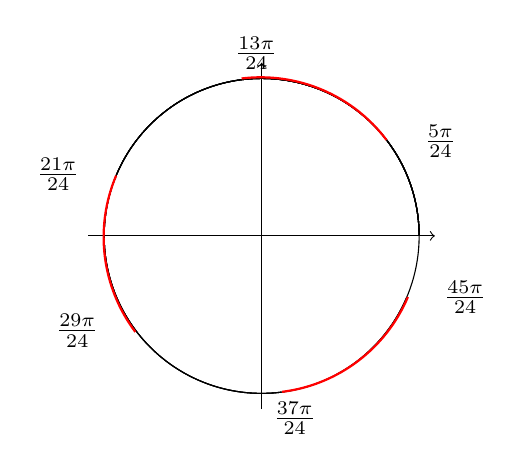
\begin{tikzpicture}[scale=2]
%Axes
\draw [->] (-1.1,0) -- (1.1,0);
\draw [->] (0,-1.1) -- (0,1.1);
%Cercle
\draw (0,0) circle (1);
%Points
\draw (1,0) arc (0:37:1) node[right] {$\quad \ddp \frac{5\pi}{24}$} ;
\draw (1,0) arc (0:97:1) node[above] {$\quad \ddp \frac{13\pi}{24}$} ;
\draw (1,0) arc (0:157:1) node[left] {$ \ddp \frac{21\pi}{24} \quad$} ;
\draw (1,0) arc (0:217:1) node[left] {$\ddp \frac{29\pi}{24}\quad $} ;
\draw (1,0) arc (0:277:1) node[below] {$\quad \ddp \frac{37\pi}{24}$} ;
\draw (1,0) arc (0:337:1) node[right] {$\quad \ddp \frac{45\pi}{24}$} ;
%Intervalles cercle
\draw [red, {[-]}, thick] (0.793,0.609) arc (37:97:1) ;
\draw [red, {[-]}, thick] (-0.924,0.383) arc (157:217:1) ;
\draw [red, {[-]}, thick] (0.13,-0.99) arc (277:337:1) ;
\end{tikzpicture}
\end{center}
\end{minipage}
On obtient finalement :
$$\fbox{$\mathcal{S}_{\lbrack 0,2\pi\lbrack}=\left\lbrack \ddp\frac{5\pi}{24},\ddp\frac{13\pi}{24}\right\rbrack\cup\left\lbrack \ddp\frac{21\pi}{24},\ddp\frac{29\pi}{24}\right\rbrack\cup\left\lbrack \ddp\frac{37\pi}{24},\ddp\frac{45\pi}{24}\right\rbrack$}.$$
Et :
$$\fbox{$\mathcal{S}_{\rbrack -\pi,\pi\rbrack}=\left\rbrack -\pi,-\ddp\frac{19\pi}{24} \right\rbrack
\cup\left\lbrack -\ddp\frac{11\pi}{24},-\ddp\frac{\pi}{8}\right\rbrack\cup\left\lbrack \ddp\frac{5\pi}{24},\ddp\frac{13\pi}{24}\right\rbrack\cup\left\lbrack \ddp\frac{21\pi}{24},\pi\right\rbrack$}.$$
%------------------------------
\item \textbf{R\'esolution de $\mathbf{\cos{(x)}+\cos{\left( x+\ddp\frac{\pi}{3}  \right)}>0     }$ $(\star)$:}\\
\noindent On obtient
$$\begin{array}{llll}
(\star)&\Leftrightarrow & 2\cos{(x+\ddp\frac{\pi}{6})}\cos{(-\ddp\frac{\pi}{6})}>0&\vsec\\
&\Leftrightarrow &\cos{(x+\ddp\frac{\pi}{6})}>0 & \hbox{car}\ 2\cos{(\ddp\frac{\pi}{6})}>0.
\end{array}$$
On s'est donc ramen\'e \`a une in\'equation fondamentale que l'on r\'esout graphiquement (\`a faire).
$$\begin{array}{lll}
(2)&\Leftrightarrow &\exists k\in\Z,\ -\ddp\frac{\pi}{2}+2k\pi<x+\ddp\frac{\pi}{6}<\ddp\frac{\pi}{2}+2k\pi\vsec\\
&\Leftrightarrow & \exists k\in\Z,\  -\ddp\frac{2\pi}{3}+2k\pi<x<\ddp\frac{\pi}{3}+2k\pi.
\end{array}$$
Ainsi on obtient :
$$\fbox{$\mathcal{S}_{\lbrack 0,2\pi\lbrack}=\left\lbrack 0,\ddp\frac{\pi}{3}\right\lbrack\cup\left\rbrack \ddp\frac{4\pi}{3},2\pi\right\lbrack\  
\hbox{et}\ \mathcal{S}_{\rbrack -\pi,\pi\rbrack}=\left\rbrack -\ddp\frac{2\pi}{3},\ddp\frac{\pi}{3}  \right\lbrack$}.$$
%------------------------------
\item \textbf{R\'esolution de $\mathbf{2\cos{(x)}-\sin{(x)}>\sin{(3x)}     }$ $(\star)$:}\\
\noindent On a
$$
(\star) \Leftrightarrow  2\cos{x}>\sin{x}+\sin{(3x)}
\Leftrightarrow  2\cos{x}>2\sin{(2x)}\cos{x}
\Leftrightarrow  \cos{x}\left\lbrack 1-\sin{(2x)}\right\rbrack >0.
$$
En remarquant qu'on a toujours $\sin{(2x)}\leq 1$, \`a savoir $1-\sin{(2x)}\geq 0$, l'in\'equation $(\star)$ est en fait \'equivalente \`a
$$
(\star)\Leftrightarrow \left\lbrace\begin{array}{l}
\cos{x}>0\vsec\\
\hbox{et}\vsec\\
1-\sin{(2x)}\not= 0
\end{array}\right.
\Leftrightarrow  \left\lbrace\begin{array}{l}
\exists k\in\Z,\ x\not= \ddp\frac{\pi}{4}+k\pi\vsec\\
\hbox{et}\vsec\\
\exists k\in\Z,\ -\ddp\frac{\pi}{2}+2k\pi<x<\ddp\frac{\pi}{2}+2k\pi
\end{array}\right. 
$$
Ainsi, on obtient:
$$ \fbox{$\mathcal{S}_{\lbrack 0,2\pi\lbrack}=\left\lbrack 0,\ddp\frac{\pi}{4}\right\lbrack\cup\left\rbrack \ddp\frac{\pi}{4},\ddp\frac{\pi}{2}\right\lbrack\cup\left\rbrack \ddp\frac{3\pi}{2},2\pi \right\lbrack\  
\hbox{et}\ \mathcal{S}_{\rbrack -\pi,\pi\rbrack}=\left\rbrack -\ddp\frac{\pi}{2},\ddp\frac{\pi}{4}  \right\lbrack\cup\left\rbrack \ddp\frac{\pi}{4},\ddp\frac{\pi}{2}  \right\lbrack$}.$$
%------------------------------
\item \textbf{R\'esolution de $\mathbf{4\cos^2{(x)}+2(\sqrt{3}-1)\sin{(x)}+\sqrt{3}-4>0  }$ $(\star)$ :}\\
\noindent On a
$$\begin{array}{lll}
(\star)&\Leftrightarrow & 4(1-\sin^2{x})+2(\sqrt{3}-1)\sin{x}+\sqrt{3}-4>0
\Leftrightarrow  -4\sin^2{x}+2(\sqrt{3}-1)\sin{x}+\sqrt{3}>0\vsec\\
&\Leftrightarrow & 4\sin^2{x}+2(1-\sqrt{3})\sin{x}-\sqrt{3}<0
\Leftrightarrow  \left\lbrace\begin{array}{l}
X=\sin{x}\vsec\\
4X^2+2(1-\sqrt{3})X-\sqrt{3}<0\ (\star\star).
\end{array}\right.
\end{array}$$
On r\'esout $(\star\star)$:\\
$$
\Delta = 4(1-\sqrt{3})^2+16\sqrt{3}
= 4\left( 1+3-2\sqrt{3}+4\sqrt{3}  \right)
= 4\left( 1+3+2\sqrt{3}    \right)
= \left\lbrack 2(1+\sqrt{3})\right\rbrack^2.$$
\noindent Les solutions sont donc $X_1=\ddp\frac{\sqrt{3}}{2}\  \hbox{et}\ X_2=-\ddp\frac{1}{2}.$
Ainsi, on obtient $(4)\Leftrightarrow -\ddp\demi < \sin{x} <\ddp\frac{\sqrt{3}}{2}.$
On s'est donc ramen\'e \`a des in\'equations fondamentales que l'on r\'esout graphiquement.\\
\begin{minipage}[c]{0.45\textwidth}
On obtient :
\conclusion{$\mathcal{S}= \ddp \mathop{\bigcup}\limits_{k \in \Z} \left( \left] -\ddp\frac{\pi}{6}+2k\pi, \ddp\frac{\pi}{3}+2k\pi \right[ \cup \left] \ddp\frac{2\pi}{3}+2k\pi, \ddp\frac{7\pi}{6}+2k\pi\right[ \right)$}.\end{minipage}

\begin{center}
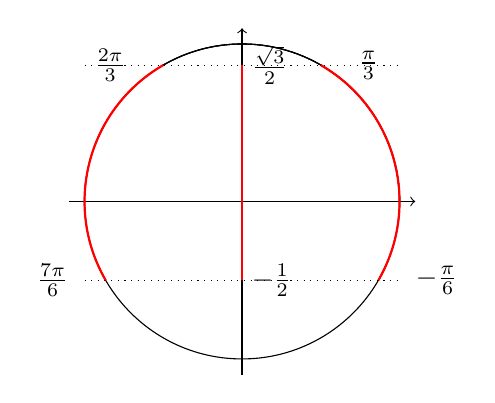
\begin{tikzpicture}[scale=2]
%Axes
\draw [->] (-1.1,0) -- (1.1,0);
\draw [->] (0,-1.1) -- (0,1.1);
%Cercle
\draw (0,0) circle (1);
%Intervalles axes
\draw [red,{]-[}, thick] (0,-0.5) -- (0,0.866) ;
%Traits
\draw [dotted] (-1,-0.5) -- (1,-0.5) ;
\draw [dotted] (-1,0.866) -- (1,0.866) ;
%Points
\draw (0,0.866) node[right] {$\ddp \frac{\sqrt{3}}{2}$};
\draw (0,-0.5) node[right] {$\ddp - \frac{1}{2}$};
\draw (1,0) arc (0:210:1) node[left] {$\ddp  \frac{7\pi}{6} \quad $} ;
\draw (1,0) arc (0:-30:1) node[right] {$\quad -\ddp \frac{\pi}{6}$} ;
\draw (1,0) arc (0:60:1) node[right] {$\quad \ddp \frac{\pi}{3}$} ;
\draw (1,0) arc (0:120:1) node[left] {$\ddp \frac{2\pi}{3}\quad $} ;
%Intervalles cercle
\draw [red, {]-[}, thick] (0.866,-0.5) arc (-30:60:1) ;
\draw [red, {]-[}, thick] (-0.5,0.866) arc (120:210:1) ;
\end{tikzpicture}
\end{center}
\end{enumerate}
\end{correction}